\begin{exercise}
      {ID-42df963f029694c68d8cf7fcfac225e8c53415e5}
      {Maximales Rechteck im gleichseitigen Dreieck}
  \ifproblem\problem
    \begin{minipage}{0.28\textwidth}
      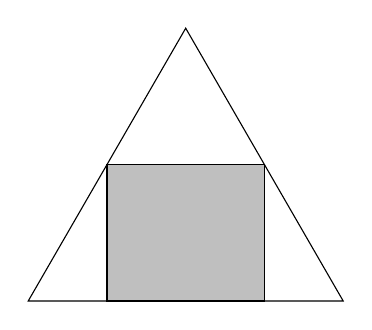
\begin{tikzpicture}
        \draw (-2.000,  0.000) -- ( 2.000,  0.000) -- ( 0.000,  3.464) -- cycle;
        \filldraw[fill=black!25!white] (-1.000,  0.000) rectangle ( 1.000,  1.732);
      \end{tikzpicture}
    \end{minipage}%
    \hfill
    \begin{minipage}{0.7\textwidth}
      Einem gleichseitigen Dreieck mit der Seitenlänge $a$ soll ein Rechteck
      einbeschrieben werden. Wie lang müssen die Rechteckseiten sein, damit der
      Flächeninhalt des Rechtecks maximal wird?
    \end{minipage}
  \fi
  %\ifoutline\outline
  %\fi
  %\ifoutcome\outcome
  %\fi
\end{exercise}
